\documentclass[12pt, a4paper]{article}
\usepackage{listings}
\usepackage[dutch]{babel}
\usepackage{array}
\usepackage{adjustbox}
\usepackage{wrapfig}
\usepackage{graphicx}
\graphicspath{{images/}}
\usepackage{chngcntr}
\counterwithin{figure}{section}
\title{Efficiëntie van raymarching in renderen}
\author{Taeke Roukema}
\date{Oktober 2022}
\begin{document}
\maketitle
\begin{abstract}
Renderen met raymarching is fucking lijp brooo. Iedereen zou het moeten doen eigenlijk.
\end{abstract}
\clearpage
\tableofcontents{}
\clearpage
\section{Voorwoord}
\clearpage
\section{Inleiding}
\subsection{Introductie onderwerp}

\paragraph{}
Renderen is overal. Als je je telefoon opent zie je allerlei gerenderde vormen. Bij het ontbijt zijn verpakkingen volgeprint met teksten die met de computer getekend zijn. Als je langs een bouwterrein loopt zie je hyperrealistische visualisaties van de architectuur. Moderne blockbuster-films zitten tegenwoordig bomvol CGI\footnote{\textbf{C}omputer \textbf{G}enerated \textbf{I}magery}. En er zijn al tientallen jaren films te zien die helemaal door de computer gemaakt zijn. 

\paragraph{}
\begin{wrapfigure}{s}{0.5\textwidth}
    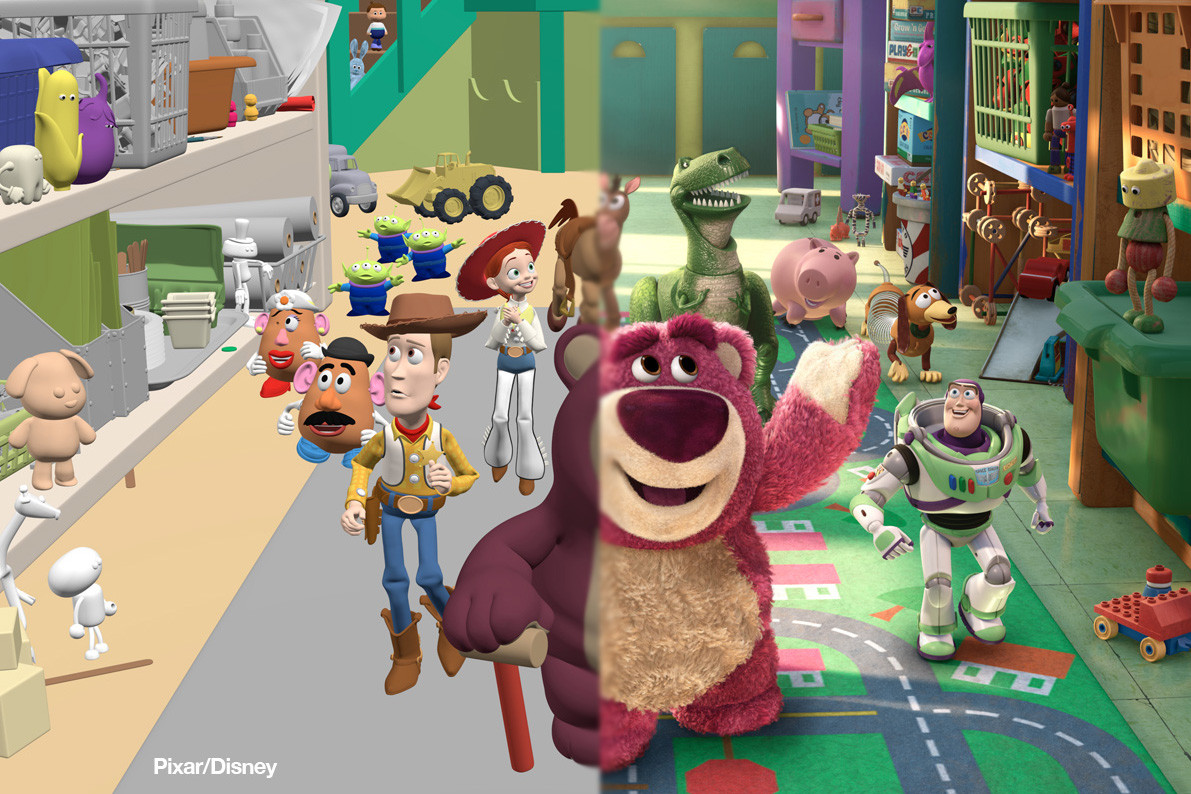
\includegraphics[width=1\linewidth]{toystory3comparison.jpg}
    \caption{Een frame uit Toy Story 3, aan de linkerkant worden geen lichtberekeningen gedaan, en aan de rechterkant wel.}
    \label{fig:toystory3}
\end{wrapfigure}
Voor Toy Story 3 (Figuur \ref{fig:toystory3}) werd er gemiddeld zeven uur over gedaan om een frame te renderen \cite{HowToyStory3WasMade}. En dat terwijl er gebruik werd gemaakt van twee gigantische render farms\footnote{Een computercluster speciaal gemaakt voor het renderen van CGI, de term was geïntroduceerd in de productie voor Bored Room\cite{MakingOfBoredRoom}}. Het renderen van films kost niet alleen enorm veel tijd, maar ook veel energie. Het is dus belangrijk dat het zo efficiënt mogelijk gebeurd. Er wordt over de hele wereld voortdurend onderzoek gedaan naar manieren om dit proces efficiënter te maken en te verbeteren. De opkomst van kunstmatige intelligentie begint al bewegingen te maken in de wereld van CGI \cite{NeRFactor}. Maar er wordt ook voortdurend voortuitgang gemaakt op fundamentelere manieren. Zo zijn er de afgelopen vijf jaar GPU's\footnote{\textbf{G}raphical \textbf{P}rogramming \textbf{U}nit} van Nvidia op de markt gekomen met ingebouwde support voor realtime raytracing\cite{NvidiaRTX}. Door op het hardware niveau de chips zo te ontwerpen dat ze heel goed zijn in bepaalde berekeningen die gebruikt worden voor het simuleren van licht kunnen GPU's gebruikt worden om voormalig minutendurende processen meer dan zestig keer per seconde uit te voeren. 
\begin{figure}[h]
    \centering
    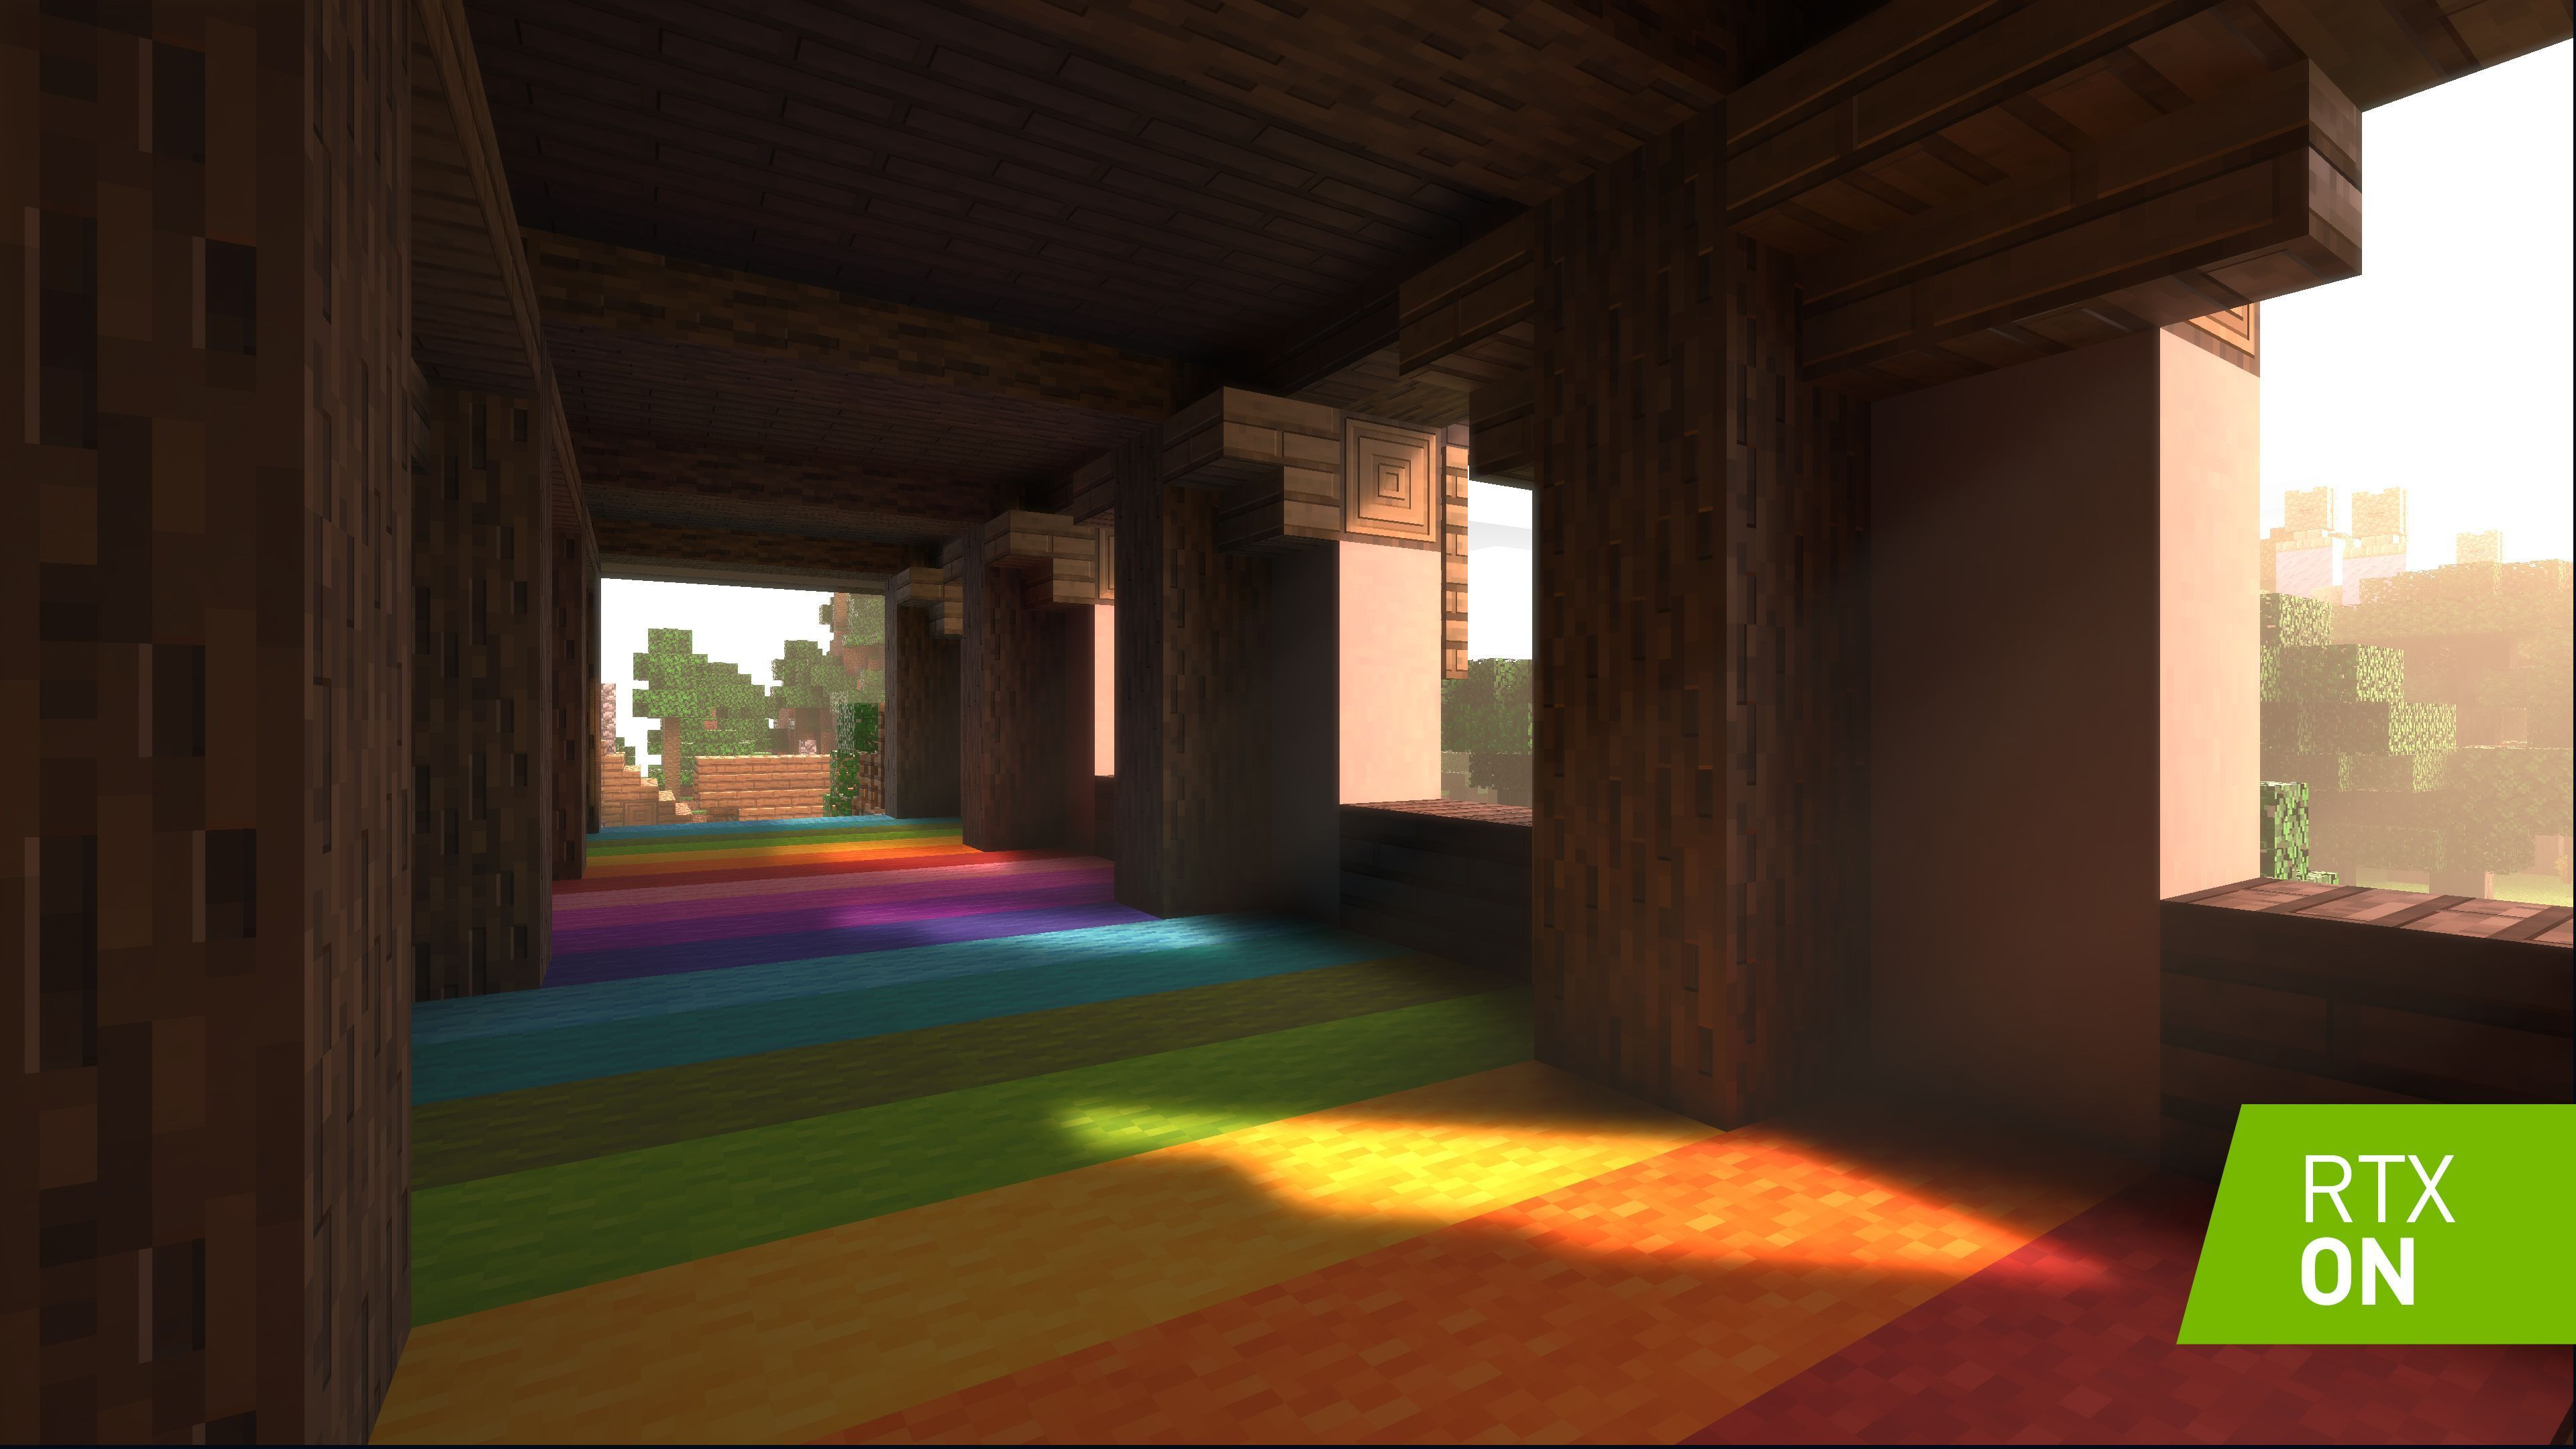
\includegraphics[width=0.5\textwidth]{minecraftrtx.jpg}
    \caption{De videogame Minecraft kan gebruik maken van Nvidia GPU's om realtime lichtsimulaties te berekenen.}
    \label{fig:minecraftrtx}
\end{figure}
\paragraph{}
Er zijn twee belangrijke maatstaffen waarmee we de efficiëntie van een renderalgoritme kunnen meten. De eerste is vanzelfsprekend: snelheid. Als een frame sneller gerenderd is wordt er minder energie gebruikt en zijn we goedkoper uit. Maar ook geheugenbezetting is belangrijk om rekening mee te houden. Het geheugen is simpelweg de plaats in de computer waar alle informatie wordt opgeslagen. Als je berekeningen doet moet je ergens de resultaten tussendoor opslaan. Complexe scènes kunnen enorm veel details hebben, die allemaal in het geheugen opgeslagen zijn. Het is niet gratis om extra geheugen toe te voegen, het is dus belangrijk om de geheugenbezetting te minimaliseren. 
\subsection{Relevantie}
Vrijwel alles is tegenwoordig op een manier gerenderd. Objecten zijn gedesigned met gebruik van CAD\footnote{\textbf{C}omputer \textbf{A}ided \textbf{D}esign}. Besturingssytemen runnen op een grafische shell. En een meerendeel van advertenties gebruikt CGI.
% Beschrijven hoe renderen voorkomt in het dagelijkse leven
% Beschrijven hoeveel energie renderen kan kosten
% Impact klimaat
\subsection{Onderzoeksvraag/deelvragen}
\clearpage
\section{Theorie}
\subsection{Wat is renderen?}
\paragraph{}
Renderen is, in feite, het weergeven van een representatie van een concept op een beeldscherm. Wij zijn voortdurend bezig met het interacteren met computers, en die interactie verloopt via het beeldscherm. Maar de computer kan uit zichzelf niet zomaar alles tekenen. Daar worden allemaal algoritmes voor geschreven. Een voorbeeld van zo'n algoritme is het tekenen van een rechthoek. In pseudocode zou je dat als volgt voor kunnen stellen:
\begin{lstlisting}[language=C]
function drawRectangle(x1, x2, y1, y2) {
	for (x = x1; x < x2; x++) {
		for (y = y1; y < y2; y++) {
			drawPixel(x, y);
		}
	}
}
\end{lstlisting}
\paragraph{}
Het algoritme beschouwt elke pixel die binnen de rechthoek valt en kleurt die pixel. In dit geval wordt dat gedaan door twee loops, die samen alle mogelijke combinaties van x- en y-coördinaten doorlopen. 

\paragraph{}
Renderen omvat, in principe, niks anders dan het aansturen van individuele pixels. Zo'n pixel heeft op de meeste moderne beeldschermen drie waarden die de kleur aansturen: R, G en B, die respectievelijk staan voor rood, groen en blauw. Ze kunnen een geheel getal tussen de 0 en 255 aannemen wat resulteert in 224 mogelijke kleuren.
\begin{figure}[h]
\centering
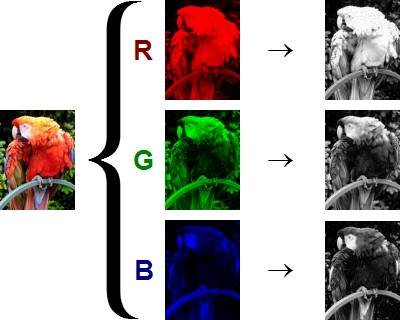
\includegraphics[width=0.5\textwidth]{RGB_channels_separation.png}
\caption{De kleuren in een foto kunnen opgesplitst worden in rode, groene en blauwe kanalen.}
\label{fig:rgb_separated}
\end{figure}

\paragraph{}
Renderen doen we op een twee-dimensionaal beeldscherm. Dat betekent dat de positie van elke pixel te beschrijven is met twee waarden. Maar de wereld om ons heen kent niet twee, maar drie ruimtelijke dimensies. Door licht dat op ons netvlies valt na weerkaatst te zijn door verschillende objecten kunnen wij die wereld representeren in onze hersenen op een tweedimensionale manier. Camera's gebruiken een gelijksoortige techniek, de lens neemt het licht en projecteert het op een sensor die de intensiteit en de kleur waarneemt. Met het renderen van driedimensionale objecten proberen we deze processen na te bootsen. 
\subsection{Wat is raytracing?}

Raytracing zou gezien kunnen worden als de meest voor de hand liggende rendermethode. Het ligt het dichtst in de buurt van het simuleren van echt licht. Het belangrijkste verschil tussen raytracen en licht in onze fysieke wereld is dat we met raytracen alleen het licht beschouwen wat zichtbaar is voor ons perspectief. Om dit te bereiken voeren we de lichtstralen niet af vanuit de lichtbron, maar vanuit de camera, vervolgens kaatsen we de straal af naar de lichtbron om te kijken hoe vel die plek zou zijn, en of er een ander object in de weg zit die een schaduw zou kunnen werpen. Op Figuur \ref{fig:raytracing_diagram} is zichtbaar hoe dat raytracen in werking gaat.

\begin{figure}[h]
    \centering
    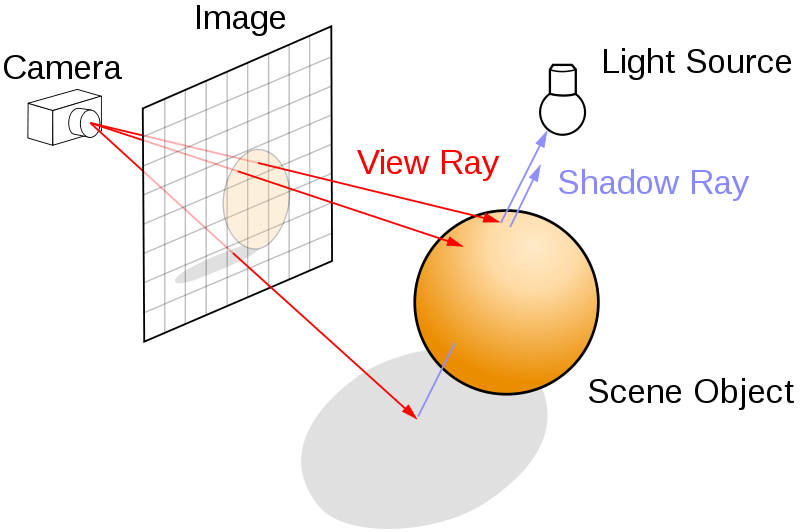
\includegraphics[width=0.75\textwidth]{raytracing_diagram.png}
    \caption{Een diagram die laat zien hoe raytracen werkt}
    \label{fig:raytracing_diagram}
\end{figure}
\subsection{Wat is rasterization?}
\subsection{Wat zijn polygonen?}
\subsection{Wat is raymarching?}
\subsection{Hoe werkt het geheugen?}
\clearpage
\section{Hypothese}
\clearpage
\section{Ontwikkeling}
\subsection{Hardware}
\subsection{Software}
\subsubsection{Besturingssysteem}
Het uitvoeren en programmeren van de code zal volledig met Linux gedaan worden. Deze keuze is om meerdere redenen gemaakt. Ten eerste is Linux de standaardkeuze voor developers om te ontwikkelen. Windows en MacOS zijn ontwikkeld als product voor de gebruiker, terwijl Linux ontwikkeld is voor stabiliteit en 	betrouwbaarheid. Dit heeft als effect dat er met Linux veel minder tegen het besturingssysteem in gewerkt hoeft te worden. Bovendien zijn alle tools die gebruikt worden voor dit onderzoek FOSS\footnote{\textbf{F}ree and \textbf{O}pen \textbf{S}ource \textbf{S}oftware}, en daardoor voor zowel Windows als Linux beschikbaar. Dus qua support maakt het geen verschil.

Als distributie\footnote{Linux zelf is slechts een \emph{kernel} die de interactie tussen de hardware en de software regelt. Bovenop deze \emph{kernel} bestaan distributies die het een werkend besturingssysteem maken.} is voor Manjaro\footnote{https://manjaro.org/} gekozen. Dit is een fork van Arch Linux. Arch Linux staat erom bekend dat het altijd de nieuwste versie van software support. Dit komt doordat het een \emph{rolling release model} heeft, in tegenstelling tot \emph{fixed release}, waar distributies zoals Debian gebruik van maken. Bovendien heeft Arch Linux toegang tot de Arch User Repository (AUR). Dat is een enorme collectie van software die gebruikers zelf kunnen uploaden naar de Arch servers, met helpers zoals \emph{yay} kan je met één commando vrijwel alle software die beschikbaar is op GNU/Linux op de computer installeren. De combinatie van deze voordelen maken Arch Linux een erg aantrekkelijke distributie om te gebruiken als programmeur. Manjaro voegt de rest van de functies toe aan het besturingssysteem, zoals een Desktop Environment (DE) en een terminal.
\subsubsection{Programmeertaal}
Er zijn talloze programmmeertalen die geschikt zijn voor graphics programming. Daarom was de keuze voor de programmeertaal niet makkelijk. Zelf heb ik al jarenlang ervaring met Python\footnote{https://www.python.org/}, maar deze taal staat niet bekend om de snelheid. Dit komt doordat het een \emph{interpreted} taal is. Dat betekent dat de code live gelezen wordt wanneer gerund. Dit staat tegenover \emph{compiled} talen, die de code eerst compileren naar machinetaal. Die machinetaal is veel efficiënter te lezen door computers, waardoor de snelheid toeneemt. Een andere optie was Javascript, het grote voordeel van deze taal is dat hij speciaal voor het web gemaakt is. Hierdoor zou het delen van het gemaakte project met anderen zo simpel zijn als het doorsturen van een url. Bovendien maakt Javascript op moderne browsers gebruik van Just In Time (JIT) compilation. Dat is een combinatie tussen \emph{interpreted} en \emph{compiled} waar de code live omgezet wordt in machinetaal voordat het gerund wordt. Maar toch is zelfs Javascript niet snel genoeg. Bovendien missen beide talen iets wat erg belangrijk is in computer graphics: controle over het geheugen. Scènes kunnen enorm complex zijn dus het is belangrijk dat die zo efficiënt mogelijk in het geheugen geplaatst worden, en het geheugen moet weer gewist worden wanneer het niet meer gebruikt wordt. Python en Javascript geven allebei niet die controle, in plaats daarvan probeert de \emph{interpreter} zelf zo efficiënt mogelijk het geheugen te gebruiken. Om deze redenen heb ik gekozen voor C++, deze taal is in 1985 uitgevonden door Brane Stroustrup en wordt vandaag de dag nog door 20,17\% van Stack Overflow gebruikers gebruikt\cite{StackOverflowSurvey}. De taal is ontwikkeld als extensie voor C, waardoor het moderne functies heeft zoals \emph{Object Oriented Programming} (OOP) en datastructuren. Maar het heeft tegelijkertijd alle voordelen die C heeft als low-level taal. 
\subsubsection{Framework}
C++ heeft uit zichzelf nog geen grafische capabiliteiten. Daar is een framework voor nodig. Moderne grafische kaarten zijn allemaal gemaakt met speciale specificaties, die ervoor zorgen dat het besturingssysteem weet hoe hij moet communiceren met de GPU. Er zijn verschillende van deze specificaties met verschillende doelen. Zo heb je DirectX, die specifiek gemaakt is voor Windows. En wat algemenere API\footnote{\textbf{A}pplication \textbf{P}rogramming \textbf{I}nterface} is OpenGL (Open Graphics Library). Met C++ is het dan ook mogelijk om direct gebruik te maken van deze API, net als in de meeste programmeertalen. 

Maar toch heb ik daar niet voor gekozen. Dit is omdat OpenGL heel goed is in het implementeren van bestaande rendermethodes, waar de GPU ook voor ontwikkeld is. Dit maakt het ideaal voor het bouwen van videogames, omdat het daar heel snel in is. Maar minder voor dit specifieke onderzoek. Ik wil objectief vergelijken hoe de verschillende rendermethoden tegen elkaar opwegen, als de gebruikelijkere methodes heel goed geoptimaliseerd zijn door de GPU en OpenGL zou dat oneerlijk zijn en de data onbetrouwbaar maken. Daarom heb ik gekozen voor raylib\footnote{https://www.raylib.com/}. Raylib is een zeer minimalistische \emph{library} die alle basistools geven die we nodig hebben om te kunnen tekenen op een canvas, terwijl het tegelijkertijd razendsnel blijft. 
\subsubsection{Integrated Development Environment}
Ik ga al mijn programmeren doen in Visual Studio Code\footnote{https://code.visualstudio.com/} omdat het een mooie simpele text editor is die precies doet wat ik wil. Het geeft goede IntelliSense\footnote{Verzamelnaam voor tools die helpen in het schrijven van code zoals: code completion en informatie over parameters}, syntax highlighting en het geeft een goed overzicht van het project. Bovendien heeft het een enorme markt van plugins die het product nog meer verbeteren. Zo gebruik ik de Vim keybinds plugin om de efficiënte workflow van de editor Vim\footnote{https://www.vim.org/} te emuleren. 
\subsection{Programmeren}
\clearpage
\section{Methode}
\subsection{Variabelen}
\subsection{Meetmethoden}
\clearpage
\section{Resultaten}
\subsection{Snelheid}
\subsection{Geheugenbezetting}
\subsection{Renders}
\clearpage
\section{Nauwkeurigheidsanalyse}
\clearpage
\section{Conclusie}
\clearpage
\section{Discussie}
\clearpage
\section{Nawoord}
Bedankt aan mijn moeder Arria Gosman.
\clearpage
\section{Literatuurlijst}
\bibliographystyle{apalike}
\bibliography{refs}
\clearpage
\section{Logboek}
\begin{adjustbox}{angle=270}
\begin{tabular}{ | c | c c c c c | }
\hline
Activiteit & Datum & Tijd (m) & Totale tijd (h) &       \% Voltooid \\
\hline
Programmeren & 20220906 & 45 & 0.8 & 0.94\% \\
Programmeren & 20220908 & 30 & 1.3 & 1.56\% \\
Gesprek met begeleider & 20220909 & 20 & 1.6 & 1.98\% \\
Programmeren & 20220921 & 90 & 3.1 & 3.85\% \\
Inhoudsopgave Opzet & 20220928 & 35 & 3.7 & 4.58\% \\
Schrijven Theorie/Achtergrond Renderen & 20220930 & 45 & 4.4 & 5.52\% \\
Opzetten \LaTeX \space Document & 20221002 & 120 & 6.4 & 8.02\% \\
\hline
\end{tabular}
\end{adjustbox}

\end{document}